\documentclass[9pt, a4paper]{IEEEtran}

\usepackage{amsmath}
\usepackage{hyperref}
\usepackage{xcolor}
\hypersetup{
    colorlinks,
    linkcolor={red!50!black},
    citecolor={blue!50!black},
    urlcolor={blue!80!black}
}

\usepackage{graphicx}
\graphicspath{ {..} }

\usepackage{tabularx}
\usepackage{caption}

\usepackage{listings}
\lstset{
    alsoletter={-},
    keywords=[1]{for, each, has, from, to, if, elif, add, del, s.t., and, break},
    keywords=[2]{edge, i, j, k, bin, bins,},
    keywordstyle=[1]{\bfseries},
    keywordstyle=[2]{\itshape},
    columns=flexible,
    mathescape
}

\author{Davide Marincione (1927757), Dario Loi (1940849)}
\title{On creating a predictor for player's movements in CSGO}

\begin{document}
    \maketitle

    \begin{abstract}
        In this document the creation of a model for predicting player's movement in "Counter Strike: Global Offensive" is described. We go on detailing the multiple problems we faced and the solutions we came up to overcome them (or the failures we couldn't surpass), starting from the very extraction of data (both from the game map and from actual matches) up to the finalization of a system that proposes possible positions for a player, given his position some seconds before.
    \end{abstract}

    \section{Grid extraction}
    To analyze and predict player's movements we first had to face the not-so-trifling matter of forming a structure upon which to execute processes, some manner of way to standardize player's behavior.

    \paragraph*{Tessellation}
    To reach this end, we realized that, even though a game of this type is \emph{almost} continuous, we had to make it discrete. Thus our first task was to tessellate the game's map (the one we chose, as we talked about in our proposal, is \texttt{de\_dust2}) into easy-to-handle bins.

    The first choice to make was on the size and shape of these bins: normally one would go straight with some manner of squares, but this time, since we didn't want to leave anything to the whims of fate, we gave a look at both the pros and cons of either using squares or hexagons to tile a map.

    \begin{itemize}
        \item \textbf{Squares}
        \begin{itemize}
            \item[Pros:]
            \begin{enumerate}
                \item Understandable at a first glance to everybody.
                \item Easy to make and navigate.
                \item Structures usually feature plants with 90 degree angles (city maps are square-y).
            \end{enumerate}
            \item[Cons:]
            \begin{enumerate}
                \item Definition of neighbor \emph{could} be argued upon (are neighbors \emph{only} those tiles which share edges or can those which share vertices also count?).
                \item Distance between center of a square and that of its (arguable) neighbor is not constant (time to get from one to the other may change).
                \item Coverage on non-axis aligned paths is poor (removing the nice part about square-y cities).
            \end{enumerate}
        \end{itemize}
        \item \textbf{Hexagons}
        \begin{itemize}
            \item[Pros:]
            \begin{enumerate}
                \item Definition of neighbor cannot be argued upon (all pieces which share a vertex also share edges).
                \item Distance from one's center and that of its neighbors is constant (\emph{may} remove some headaches down the road, early optimization).
                \item Coverage on some paths is still poor, but at least less so than squares (assuming comparable size of tiles).
                \item Polygon with the most number of edges capable of tiling a plane by itself: hence best proxy for a circle, a pretty important thing when agents can move in any direction.
                \item Fancy.
            \end{enumerate}
            \item[Cons:]
            \begin{enumerate}
                \item Less understandable... but it is still a hexagon tiling, so not too much.
                \item Less easy to make (not too much).
                \item Fits less nicely some plants.
            \end{enumerate}
        \end{itemize}
    \end{itemize}

    As some may have already guessed, our choice landed on the hexagons.

    Having decided how to deal with the map, we had to get its terrain data from somewhere: for sure we weren't going to scour the internet for dubiously sourced files nor did we have the time to learn Hammer\footnote{The software used to make maps for Source games} to extract the data ourselves by reverse engineering the map from the game's files.
    Fortunately though the paper \textbf{Valuing Player's Actions in Counter-Strike: Global Offensive} already extracted the bot's navmesh data, which, as luck would have it, was easily attainable through the \texttt{awpy} library.

    \begin{figure}[h]
        \caption{\texttt{de\_dust2}'s navmeshes}
        \centering
        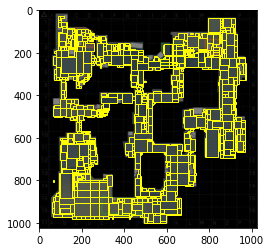
\includegraphics[width=0.4\textwidth]{images/navmeshes.png}
    \end{figure}

    This navmesh is a collection of quads (squares in 3d graphics): each quad is defined via two 3d points (its bottom left and upper right corners) and a label (the area which it is part of).


    \paragraph*{Dealing with the navmesh} Of course though we couldn't use this data completely raw, we had to repurpose it into our tiling. To do so we resolved into creating an algorithm that, given some min/max bounds and a step-value, forms the \emph{proposal} for an hexagon by checking the aforementioned navmesh data for collisions with the center of this hexagon to any mesh in the structure; if no collision is found, then it checks for collisions in its vicinity and, if a sufficiently near mesh is found, the proposal is created anyway, otherwise not.

    \paragraph*{Three dimensions}
    Now we reached our first problem: we are checking for collisions via "ray-casts" coming directly from above the map\dots then what about those layers which, topographically, intersect with each other on the map? We had to deal with this matter too, and this fact that height must be added to the calculation was a pretty huge problem, for two reasons:

    \begin{enumerate}
        \item Player's movement becomes more asymmetric: one cannot jump from road-level up to a balcony as easy as another would (conversely) leap from it.
        \item This navmesh that we used to get terrain data has pretty poor (and sometimes non-existant) height values.
    \end{enumerate}

    Thus the existance of multiple layers (but also the proposal for hexagons which do not directly collide with an actual mesh, but are just near it) lead to a problem of conflicts in the existance of hexagons on the same $(x,y)$ pair. We'll explain how we dealt with this problem a bit further down this section, but what we first want to talk about is the matter that, as said, height-data from this source is pretty poor. Why? The reason is that, for each quad, we are just given the height for its bottom left and the upper right corners, not for any other point! To have the height for \textbf{all} the points would be useless (and impossible, continuous spaces and all of that) of course, but, for our computations, the height for the other two corners is needed, because that data is fundamental if we want to apply triangle interpolation on the mesh (to find the actual height for the exact point we are checking).
    
    Some of these heights can be recovered by using neighboring quads, while some others cannot (depending on whether there exists a neighboring quad in the first place).

    To circumvent this problem we went ahead and decided two things: first we would apply some mathematical heuristics where data was unavailable, secondly, since we \emph{extensively} know the map, if further and more nuanced issues were going to arise (and they would) we would be solving them by anthropomorphic heuristics- eyeballing.

    We divided the problem in three cases:

    \begin{enumerate}
        \item Both heights can be found, no problem.
        \item One of the two heights was unavailable, not too bad.
        \item Neither height can be retrieved.
    \end{enumerate}

    In the first case of course nothing was to be done.
    In the second one we resolved in find the height of the other point by doing:

    \begin{align*}
            z_m &= \frac{z_{p_1} + z_{p_2}}{2}\\
            z_u &= 2z_m - z_k
    \end{align*}
    
    Where $z_m$ is the height of the terrain in the very middle of the quad, easily computed since we can use both heights we surely hold, $z_k$ is the known height and $z_u$ is instead the approximation for the unknown one.

    In the third and worse case otherwise we resolved in letting:

    \begin{equation*}
        z_{u_1} = z_{u_2} = z_m
    \end{equation*}

    Which is not a problem if the quad is plateaued, but is otherwise problematic when strongly angled.
    Fortunately though we kept track of all of these "bad" quads and their number amounted to roughly 30 over 1200 areas circa, hence we can assume that most of the heights were well-defined.

    As previously stated, conflict in some points for height taken from different quads was unavoidable, hence we resolved in dividing these in further three cases:
    
    \begin{enumerate}
        \item All of the quads from which the point/bin got the height are from the same area (they share the same label): average them out.
        \item The point has heights from quads of two different areas: do the mean for each label and then check the difference between the two means, if it is lower than 90 units (the maximum jumping height in-game is around 70 units) then get the lower mean (and its label) and use that, otherwise create two different points at the same x,y coordinates (one will overlay the other).
        \item The point has heights from quads of more than two different areas: make the mean for each label and then query the user (me) for decision making.
    \end{enumerate}

    \newpage

    Leaving us with the rough tiling:
    
    \begin{figure}[h]
        \caption{Pre-cleaning tiling}
        \centering
        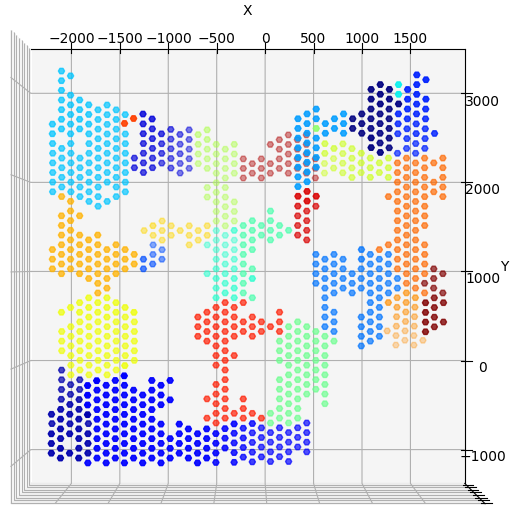
\includegraphics[width=0.2\textwidth]{images/orig_tiling1.png}
        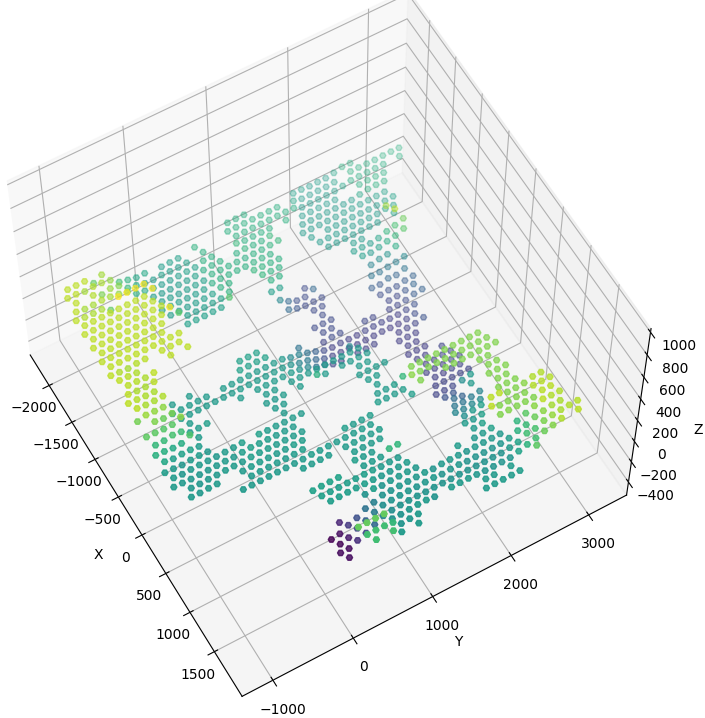
\includegraphics[width=0.2\textwidth]{images/orig_tiling2.png}
    \end{figure}

    Which, with a lot of patience as our weapon, we then manually cleaned:

    \begin{figure}[h]
        \caption{Post-cleaning tiling}
        \centering
        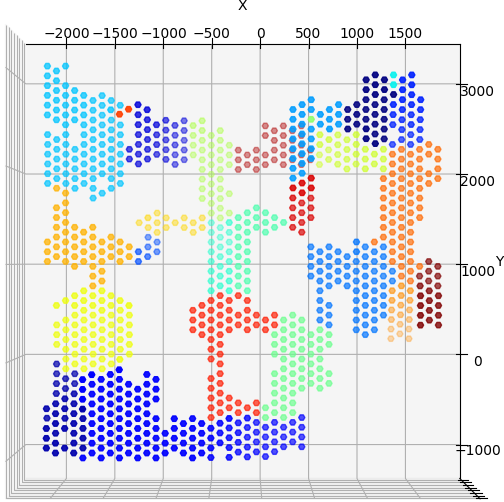
\includegraphics[width=0.2\textwidth]{images/post_tiling1.png}
        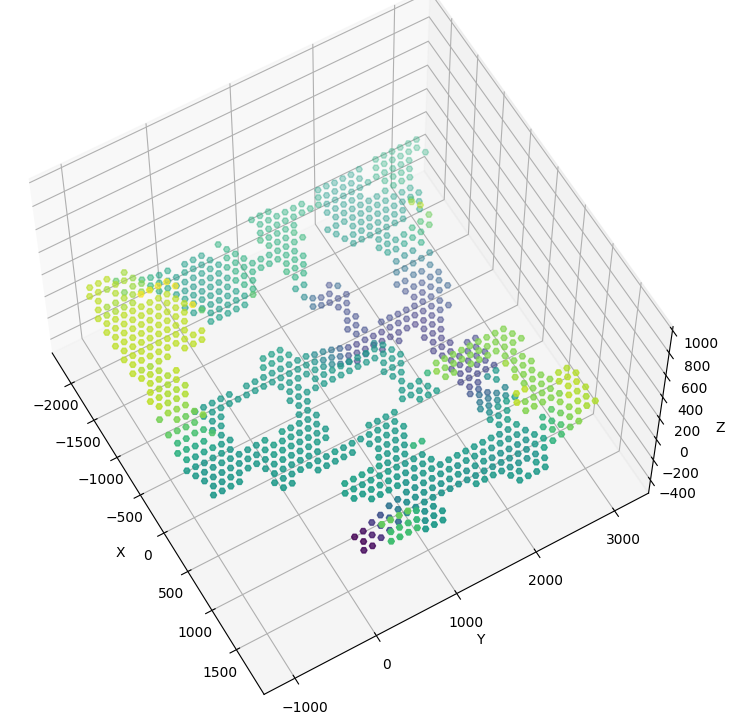
\includegraphics[width=0.2\textwidth]{images/post_tiling2.png}
    \end{figure}

    \section{Graph and vision}

    \paragraph*{Making the graph}
    Once this matter of tiling the map was solved we went ahead and started laying the bricks for our actual work, we built a model for the movement. To do so we resorted to graphs, more precisely our idea was to define a directed graph to represent the possibility of movement from one bin to another (our main learning target, more on that on other sections of the document).

    We wrote an algorithm that fills an adjacency-matrix by following\footnote{The actual code is slightly different, but this pseudo-code has the same spirit}:
    \begin{lstlisting}
for each i,j bins s.t. i$\neq$j:
    if $h_j - h_i < 70$:
        o := -1
        for each k s.t. $\exists$ i$\to$ k:
            if $x_k$ = $x_j$ and $y_k$ = $y_j$:
                o := k
                break
        if o = -1:
            add i$\to$ j
        elif $h_o$ < $h_j$:
            del i$\to$ o
            add i$\to$ j
    \end{lstlisting}

    \newpage
    After a couple of manual adjustments, we got:

    \begin{figure}[h]
        \caption{The graph}
        \centering
        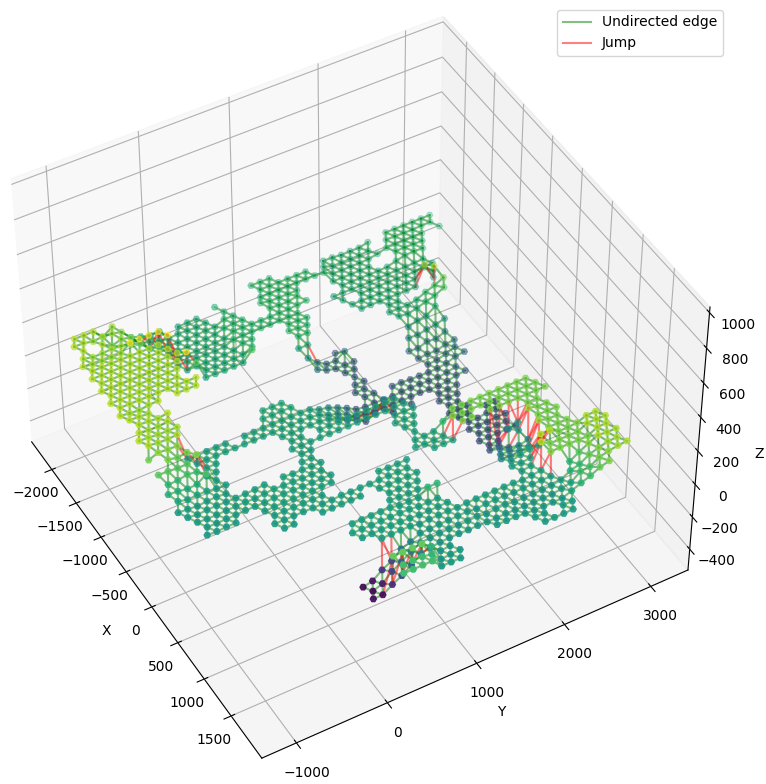
\includegraphics[width=0.44\textwidth]{images/graph.png}
    \end{figure}

    This may not seem like so big of an achievement, but to reach such refined data by just using some clever heuristics and linear algebra was extremely satisfying.

    \paragraph*{A futile quest for sight}
    Now that we had built our frame we wanted to make something more: we wanted to also create a manner of structure for a player's line-of-sight.

    The idea was that, by knowing from each bin which other bin could be seen, we could completely remove those bins from the possibilities once we started predicting where a player went.
    
    To do so we thought about going back to the navmesh data, inferring the positions of the visual obstacles (buildings, crates, vases, cars and all of those objects positioned around the map) and then doing a brute-force algorithm where we would ray-cast from one bin to the other and, if no collision was detected, the line-of-sight would be clear\dots obviously this was too nice of an idea. We realized it would've entailed a recreation of the map from scratch, something that we really didn't want to (and couldn't) do.
    Thus, as we did before, we relied on good ol' anthropomorphic heuristics\dots for each bin to each bin: in our graph there are roughly 970 bins. This quest took us a couple of weeks, and in the end we managed to get this nice simulation of a player's line of sight:

    \begin{figure}[h]
        \caption{Line-of-sight examples}
        \centering
        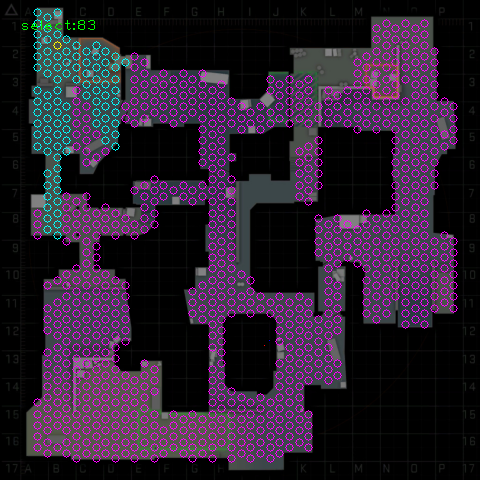
\includegraphics[width=0.2\textwidth]{images/view_B.png}
        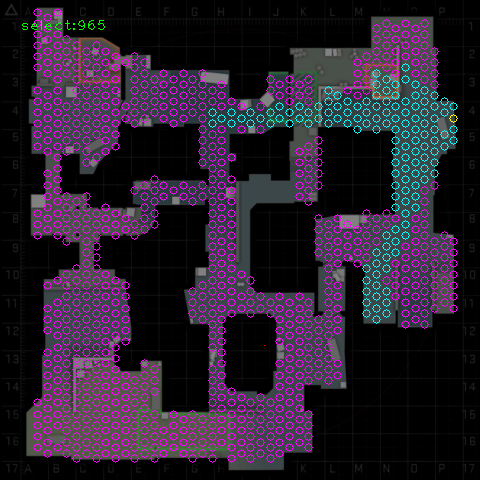
\includegraphics[width=0.2\textwidth]{images/view_car.png}
    \end{figure}

    \section{The theory}
    Before going into describing how we actually collected the data, we want to describe the theory behind our system (which we realized too late looks a lot like the special case of a Markov chain\dots we aren't \emph{that} knowledgeable on them thus we won't ever mention them again in this document).

    Here's what we know, based on how we built our frame for each cell there exists a limited number of movements that can be done: either remain on the current cell (option zero) or move to a neighboring cell (ranging from $1$ to a maximum of $6$) to which it has an assigned movement (we remind that movement isn't symmetric, thus going from $A$ to $B$ doesn't entail that one may be able to do the reverse).
    
    Our aim is to learn the average distribution of this movement given a set of explanatory variables, we think that through that we'll be able to predict (propose a range of) the position of a player by recursively applying the law of total expectation over the possible movements of the player.

    Let us explain: say we know that a player, at step $0$, goes from a cell (one of our hexagons) $K_0$ to another $K_1$. Assuming this movement is mapped in our graph then we can say for certain that this player is in cell $K_1$ thanks to movement $K_0\to K_1$, but, once we've seen that, that player goes out of our sight, thus his whereabouts are now unknown, what we want to do now is predict his movement in the next step $1$ via the range of actions we built in the previous sections.
    
    We know that this cell $K_1$ has four neighbors to which a movement \emph{is} possible (notice how we didn't include $K_0$, we'll assume $K_1\to K_0$ is not possible), $A$, $B$, $C$ and $D$. What we would like to know (what we'll have to find) is the probability where, when a player does some action $K_0 \to K_1$, he will go next, aka the conditional probability distribution for his next position.
    
    \begin{equation*}
        \mathbf{E}\left( \mathbf{P}\left(K_2\right) | K_0 \to K_1\right) =
        \begin{cases}
            \mathbf{P}\left(K_2 = K_1\right)\\
            \mathbf{P}\left(K_2 = A\right)\\
            \mathbf{P}\left(K_2 = B\right)\\
            \dots
        \end{cases}
    \end{equation*}

    The decision for what explanatory variables we used is a discussion left for the next section, now we want to explain what we do next (indeed we could give no explanatory variables in this example, but we feel like it would be a bit bare).

    Once we have this we might ask: what about the movement for step $2$? Well the answer is easy enough (the execution less), assuming we have a model for each cell then we can describe the distribution for position $K_3$ of that player as:

    \begin{align*}
        &\mathbf{E}\left( \mathbf{P}\left(K_3\right) | K_0 \to K_1\right) =\\
        \sum_{n \in N_{K_1}} &\mathbf{E}\left( \mathbf{P}\left(K_3\right)  | K_1 \to n\right)\cdot\mathbf{E}\left(\mathrm{P}(K_2 = n) | K_0 \to K_1\right)
    \end{align*}

    Where $n$ is a neighbor of $K_1$. Without loss of generality, one can easily see how this pattern could be extended to any $i$ number of steps, the only matter is that of \textbf{exploding} size of the computation. Because, if we assume the maximum number of actions per cell to be $7$, then it is trivial to prove that this computation would hold $O(7^i)$ components in the end: \textbf{not} nice.

    How did we solve this \emph{little} problem? We'll explain it in the last section, where we describe the implementation (spoiler: heuristics).

    \section{Data collection and cleaning}
    In this section we'll look at two open wounds of this project: we couldn't collect the data by ourselves and the line-of-sight system was, ultimately, useless.

    \paragraph*{Data collection} First let us explain how we were \emph{meant} to collect the data: our idea was to call a bunch of our friends and some of our colleagues and, in the span of a couple of days worth of play (we thought something like 10 hours) we would record a bunch or games (a game lasts about an hour and a single round is between one and three minutes).
    The problem? Real life got in the way, we had a lot of projects too fill out and so did our colleagues and, furthermore, most of our friends which aren't part of this course are in university, thus they too had their hands filled... what to do?

    First of all: cry a bit, because we had already built and tested our own plugin to run on a custom server (took us some days, and to learn a 20 year old and almost unused \href{https://developer.valvesoftware.com/wiki/Squirrel}{programming language}). To describe it simply, the plugin was to, at the end of every round, reshuffle the team compositions and randomize the money each player would hold by selecting it from a table of preset possible situations... alas this thing wasn't meant to be and lead to a waste of time\dots 
    
    Fortunately this game is played \textbf{a lot} on a competitive level: there's so many replay files of pro-level matches online that one could fill multiple HDDs. What we had to do was just scouring the internet for a bit and decide on the best source for our files: we landed our choice on \href{https://www.hltv.org/}{\emph{HLTV.org}} which we already knew a bit, it is the most important site when it comes to competitive CSGO after all... From this site we got a total of sixteen (16) matches between different teams on our map of choice, ten of those we used for the regression of our model, while the other six were used as test data.
    In hindsight this result was probably for the best: to be able to get the same amount data as we did like this by collecting it ourselves would've required a massive operation, one which we wouldn't have had the means to follow through with. And, as you'll see, not even all of this data was enough!

    \paragraph*{Data cleaning} Once we had downloaded our files it was time to extract relevant data from them, first thing first we decided that, since all of these replay files had to be parsed and, somewhat, discretized in terms of time (by the library, not by us, fortunately) our time-frame for the steps defined in the above theory would be, for each step, 0.5 seconds, which, for our target of predicting up to 5 seconds into the future, seemed pretty nice (strangely enough, it was!).
    
    Here's where the tears start coming out a second time though: once we started digging really deep into the functionalities of the libraries that we were meant to use we found out something. It is \href{https://pkg.go.dev/github.com/markus-wa/demoinfocs-golang/v2/pkg/demoinfocs}{\emph{impossible} (check the end of the page)} to tell whether a player is looking at another player during a step, thus we had:
    \begin{itemize}
        \item No way to validate our line-of-sight system (would've loved to since we were sure to have made mistakes).
        \item No way to tell whether a player was spotted in the first place.
    \end{itemize}
    Thus we had to scrap the idea of making use of the system\dots a full week of work down the drain (and \emph{several} bad-words in the air).

    With our dreams a bit broken, we resolved to make good use of the cards we had been dealt, and thus we followed by creating an algorithm that, given a \texttt{.json} version of the replay (the conversion from \texttt{.demo} format to \texttt{.json} is a black box solved by \texttt{awpy} for us), collects the samples we are interested in: to do so it does two passages upon our data, a first one to group it with every other sample of a player passing through that same cell and a second one, cell per cell, which actually goes through each instance of a passage through that cell and recovers our variables:

    \begin{itemize}
        \item The next movement of the player (our response variable).
        \item The player's team.
        \item The previous movement (either one of the inward movements or the current cell).
        \item The direction, with respect to the current player, of his team's center of mass.
        \item The number of his teammates alive.
    \end{itemize}

    For the regression dataset we collected the variables in groups of single frames, while in the case of the data for the test we collected them in groups of ten, since we wanted to predict the position in a timespan of five seconds (and one frame is $0.5$ seconds in our system).

    How many samples did we gather in the end? Around $540'000$ samples for the regression and $390'000$ for testing (pretty big\dots you'll soon see they were \textbf{not} enough). 

    \section{The predictor}
    Now that we had collected the data, it was time to make use of it, first of all we gave a look at a count, for each cell, of how many samples there are.

    \begin{figure}[h]
        \caption{Samples count per cell}
        \centering
        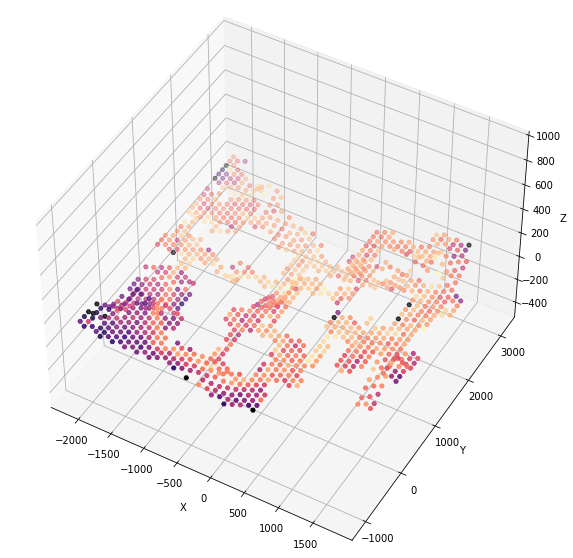
\includegraphics[width=0.44\textwidth]{images/samples_count.png}
    \end{figure}

    As expected, cells are visited with different frequency (who would've guessed, players don't stand uniformly on the map!) and there are some which are essentially unused.
    Alas, this is troubling: as we know, the more variables we fit into a regressor (the more complex we make it), the more data we need to feed it and, since we are handling a lot of categorical variables, we know that for each category that an explanatory variable can have, in reality we are adding another variable (because of the encoding). How did we solve this conundrum? With a bit of a clever "sweep under the rug" solution: we "bagged" different regressors!

    Of course the creation of different regressors is a must when doing this kind of things, but usually we would expect to just that one, after doing the checks, which best fits our case (aka, has good enough performance while using the less number of variables as possible). In this case though we had to get a bit creative: firstly our problem requires us to fit a model \emph{for each} cell\footnote{Except those which are completely unused.} and secondly it requires us to make it as \emph{powerful} as possible, if an explanatory variable can be used, we use it; the reasoning being that, since we have to predict with 10 steps into the future, we need to explain as much of the variance as possible (and since adding explanatory variables can only make our $R^2$ monotonically increase, we add them).

    What was our "pipeline" then? We prepared the formulas for five different regressors (in reality we did more for testing purposes, but in part we forgot about them and in other part they were really crazy, more on that soon) and, for each of these formulae, and each of the cells, we tried to fit a statsmodel's \texttt{MNLogit}. If statsmodel was able to fit it, then we would store the result in a vector (which we then saved as one of those \texttt{pickle}'s we'll upload along the other files), otherwise we would put a \texttt{None} instead. The models that we regressed are:

    \begin{enumerate}
        \item \texttt{choice \raisebox{-0.7ex}{\textasciitilde} 1} (the null, of course)
        \item \texttt{choice \raisebox{-0.7ex}{\textasciitilde} team}
        \item \texttt{choice \raisebox{-0.7ex}{\textasciitilde} cell\_from}
        \item \texttt{choice \raisebox{-0.7ex}{\textasciitilde} cell\_from * team}
        \item \texttt{choice \raisebox{-0.7ex}{\textasciitilde} cell\_from * team + dir\_team}
    \end{enumerate}

    As said before, we also tried other models, like:

    \begin{itemize}
        \item \texttt{choice \raisebox{-0.7ex}{\textasciitilde} cell\_from * team + n\_alive * dir\_team}
        \item \texttt{choice \raisebox{-0.7ex}{\textasciitilde} cell\_from * team * n\_alive * dir\_team}
    \end{itemize}

    But: the first just resulted in, after a number of hours, just two successful regressions (over our 967 cells), while the other\dots we stopped it after roughly eight ($8$) hours of Davide's CPU going at $100\%$ utilization (let's not talk about electricity bills).

    Once all of these models were fitted, we wanted to compare them and see \emph{how} good they are: to do so, as we said earlier, we decided on comparing their $R^2$s. Alas the no-free-lunch theorem is no joke. First of all statsmodel's returned $R^2$ for \texttt{MNLogit} is not the usual $R^2$, but is instead McFadden's \emph{pseudo}-$R^2$ (which we'll refer with $\rho^2$ from now on). Computed as:
    \begin{equation*}
        \rho^2 = 1 - \frac{\log L_c}{\log L_\mathrm{null}}
    \end{equation*}
    Secondly we couldn't use directly the $\rho^2$s to compare the different models, the reason being twofold:

    \begin{enumerate}
        \item For each formulae we have a different number of models, one for each cell (if the fit was successful).
        \item Even for the same model, cells can have a different number of explanatory variables used, because every cell may have a different number of actions assigned (since it can have a different number of neighbors).
    \end{enumerate}
    The result of these two things? We had to find out how to make an \emph{adjusted} McFadden's \emph{pseudo}-$R^2$ (had to write it in full at least once, from now on we'll call it $\rho^2_a$), which is computed as:

    \begin{equation*}
        \rho^2_a = 1 - \frac{\log\left(L_c\right) - K}{\log L_\mathrm{null}} = \rho^2 + \frac{K}{\log L_\mathrm{null}}
    \end{equation*}
    Where $K$ is the number of explanatory variables used in the model.
    Furthermore, instead of directly using these adjusted values, we had to average them: we don't know if this was the right course of action, but it seemed the most sane one.
    The results of our calculations were (numbers are related to the models we enumerated earlier):
    \begin{table}
        \centering
        \begin{tabularx}{.27\textwidth}{l c c c}
            Model\# & Fit cells & $\overline{\rho}^2$ & $\overline{\rho}^2_a$ \\
            \hline
            1\footnote{Obviously this is zero} & 945 & $0.00$ & $0.00$ \\
            2 & 885 & $0.05$ & $0.03$ \\
            3 & 741 & $0.21$ & $0.19$ \\
            4 & 477 & $0.23$ & $0.20$ \\
            5 & 503\footnote{We aren't sure why this value is higher than that of 4,\\for reasons which will be clear later we won't explore this further.} & $0.25$ & $0.21$
        \end{tabularx}
    \end{table}

    These results may seem a bit low but:

    \begin{itemize}
        \item As we know, an $R^2$ in general doesn't \textbf{have} to be high for the system using it to be regarded as good, it is just nice for it to be so.
        \item On page 35 \href{https://cowles.yale.edu/sites/default/files/files/pub/d04/d0474.pdf}{of one of his works}\footnote{No, we didn't read it to the fullest, we don't have the luxury of having so much spare time.}, McFadden himself calls a value between $0.2$ and $0.4$ for the $\rho^2$  an \emph{excellent} fit.
    \end{itemize}
    Thus we were pretty happy about it.

    Finally, since we thought it right for just one model to be used per cell, we ensembled all of these results into a single system where, if the better model is not present, then a lower level one is used, trickling down until the null model.
    From all of this we managed to get a model composed of:
    \begin{center}
        \begin{tabular} {l c c c}
            Model\# & Cells present & $\overline{\rho}^2$ (present) & $\overline{\rho}^2_a$ (present)\\
            \hline
            1 & 43 & $0.00$ & $0.00$\\
            2 & 161 & $0.11$ & $0.01$\\
            3 & 264 & $0.25$ & $0.22$\\
            4 & 477 & $0.23$ & $0.20$\\
            \hline
            Tot & 945 & $0.20$ & $0.17$
        \end{tabular}
    \end{center}

    One might ask "Hey, where's the \emph{best} model, the number 5?", we'll talk about that in a minute.

    \begin{figure}[h]
        \caption{Final ensemble capabilities}
        \centering
        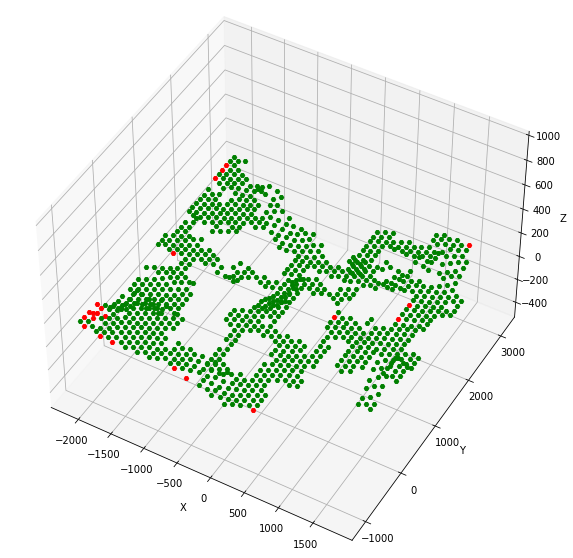
\includegraphics[width=0.44\textwidth]{images/existent_models.png}
        \caption*{In red the cells for which no fitted model exists}
    \end{figure}

    First let us talk about these numbers: each of these (except for the last total ones, which are simple averages over all cells) is \textbf{not} a copy from the previous table, but instead an average over the \textbf{present} models, aka those models which actually got into the final ensemble. Furthermore, we would like to address an interesting result: we can see that the $\overline{\rho}^2$ for the third model seems to do better than that for fourth model. The reasoning is simple: all of these averages, since they are not for the same set of cells (thus for the same set of problems), shouldn't be compared against each other, whereas we can do that in the previous table because their sets overlap (somewhat, if we don't care about the non-existent fits\dots take that table too with a grain of salt).

    Now that we had created our ensemble it was time to put it to use, to put in practice the calculations we talked about in the previous sections (and to explain why the fifth model-type wasn't cut for our purposes).

    As you'll see this algorithm is not \emph{canonical}, in the sense that it doesn't exactly apply the law of total expectation, as we said, to do that it would take $O(7^d)$ operations, something that we really wouldn't like to do. Instead what this algorithm applies is: a heuristic (a cutoff) and a method to avoid, in general (even more so when multiple predictions are done), to recompute very slow computations: \href{https://en.wikipedia.org/wiki/Memoization}{memoization} (for which already a result was given).

    From this very last method stems the reason why we couldn't apply our fifth model, because the direction of the team's center of mass is a continuous value! And, since memoization uses a map, and maps require values to be hashable, one cannot hash a continuous value into a map and hope to get the mapped result back, continuous values are rarely exactly equal to each other!

    Without writing the actual code (which you can view in the fourth \texttt{.ipynb} we've uploaded), let us describe the machinery we built as a set of steps:

    \begin{center}
        \rule{.44\textwidth}{0.4pt}
    \end{center}
    \noindent
    \textbf{\textsc{PredictMovement}}\\
    \textbf{Input}: the current cell $k$, the cell from which the player came from $f$, his team $t$, a dictionary $m$, the current depth $d$ and a cutoff value $c$.\\
    \textbf{Output}: a dictionary.
    \begin{enumerate}
        \item Create an empty dictionary $r$.
        \item If the ensemble at $k$ is \texttt{None}, return $r$.
        \item Check whether $m$[$k$,$f$,$t$,$d$] returns a dictionary, if so return that (this is called \href{https://en.wikipedia.org/wiki/Memoization}{memoization}, we'll talk about that later).
        \item From the ensemble at $k$, given the pair $\langle f, t\rangle$, get the expected distribution $p$ for the next actions $k \to A$.
        \item Sort in ascending order the distribution $p$.
        \item Check iteratively $p$: cut all the actions with probability lower than $c$, if they are cut, redistribute immediately and uniformly their probability to all the other remaining actions.
        \item For all the remaining actions $k \to a$ and their probability $p_a$:
        \begin{enumerate}
            \item If $d > 0$ then $r' =$ \textbf{\textsc{PredictMovement}}($a$, $k$, $t$, $m$, $d - 1$, $c$), otherwise $r'[a] = 1$.
            \item For all $r'[k'] = p'$ let $r[k'] = r[k'] + p' \cdot p_a$.
        \end{enumerate}
        \item Let $m$[$k$,$f$,$t$,$d$] $= r$.
        \item Return $r$.
    \end{enumerate}
    \begin{center}
        \rule{.44\textwidth}{0.4pt}
    \end{center}

    Now that all of the system was in place: we started checking it against the test data, the resulting dictionaries stored in a final file \texttt{predictions.pickle}.

    The resulting dictionaries have, for each proposed cell, a value between 0 and 1 and, furthermore, if we sum all of these together, we should get back 1 (or some floating point value near it). Thus, for all intents and purposes, each dictionary can be seen as a distribution for the player's position; what to do with these? If we visualize even one of these distributions we'll notice how they have a wildfire-like distribution, with hints of more concentrated probabilities around \emph{some} cells.

    This is pretty nice, since it means we can say, with high certainty, that the player will be in that distribution, but the question then becomes \emph{where?} Since these distributions are pretty big, they are losing a bit of meaning: in some sense, the prediction has high accuracy but low power. To address this problem we decided to add a \emph{"hyperparameter"}- instead of taking the whole distribution, we sort the values in descending order and, by summing iteratively the values up, we get all of them until an \emph{accumulation} value is reached.

    Of course though the question now becomes: what accumulation value should we choose? To answer this we crunched the numbers a little bit and came up with (the lines are averaged over the test data):

    \begin{figure}[h]
        \caption{Proposal size (left side) vs accuracy (right side)}
        \centering
        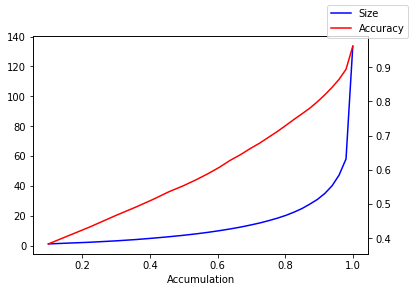
\includegraphics[width=0.44\textwidth]{images/size_v_accuracy.png}
    \end{figure}

    By gut feeling (and a bit of \emph{elbow method}) we decided that an accumulation of $.7$ \emph{should} give the right compromise between these two parameters.

    \begin{figure}[h]
        \caption{Same predictions w/out accumulation and w/ accumulation}
        \centering
        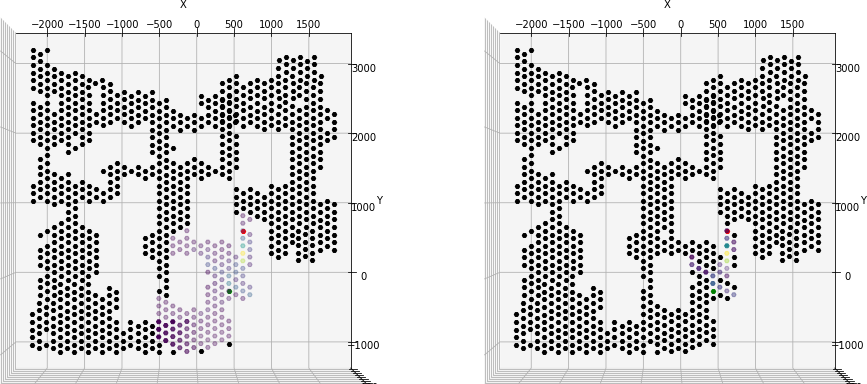
\includegraphics[width=0.44\textwidth]{images/wildfire_v_non.png}\\
        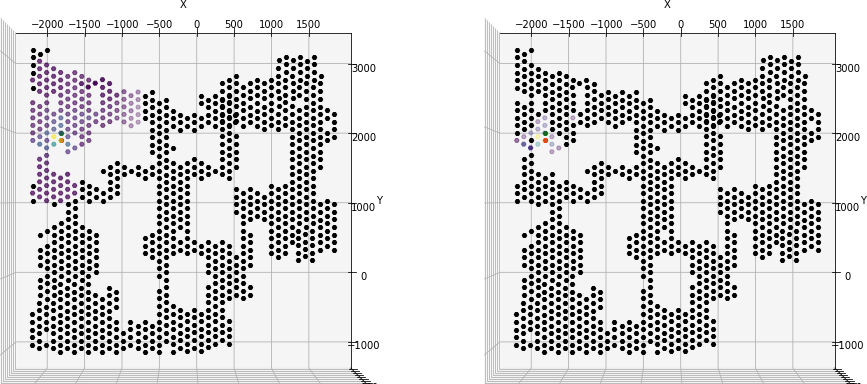
\includegraphics[width=0.44\textwidth]{images/wildfire_v_non2.png}
        \caption*{Green cell is starting, red cell is final position}
    \end{figure}

    \section{Conclusions}
    And thus this project has come to its finalization, fittingly, we don't have a single answer on the quality of our machinery: if one wants to have more assurance that the proposal will contain the player's position he can just increase the accumulation, if otherwise he wants greater pin point positioning he should accept a lower accuracy. As everything, there are compromises to be made.

    It was a pretty long, but also fun and, of course, educational experience, we hope to have satisfied our readers (and thus the professors, but also whoever will get their hands on this piece of paper).
\end{document}
